\documentclass[prl, article, twocolumn]{revtex4-1}

% packages
\usepackage[utf8]{inputenc}
\usepackage{graphicx}
\usepackage{amsmath}
\usepackage{amssymb}
\usepackage{subcaption}
\usepackage{minted}
\usepackage{fancyvrb}
\usepackage[makeroom]{cancel}

% title
\begin{document}

\title{Mini deep-learning framework}
\date{\today}
\author{Austin Zadoks}
\noaffiliation

\begin{abstract}
Popular deep learning libraries like PyTorch and TensorFlow are enormous and complex but are relatively easy to use. Therefore, many scientists and engineers eschew writing their own frameworks in lieu of using these highly available, performant, and powerful community-developed packages. Nevertheless, it is informative as a student of deep learning to implement basic functionality by hand to better understand the inner workings of deep networks (DN). Here, I present an implementation of a miniature deep-learning framework which supports fully-connected (FC) linear layers, hyperbolic tangent ($\tanh$) and rectified linear unit (ReLU) non-linear activation, stochastic gradient descent (SGD) optimization, and mean-squared error (MSE) loss. I demonstrate its performance by implementing a FC DN which predicts if a point is within a circle, and I compare the performance of $\tanh$ and ReLU activation. After 50 epochs of training, the ReLU model achieves 6.3~$\pm$~2.6~\% training error in 0.6~$\pm$~0.1~seconds, and the $\tanh$ model achieves 6.2~$\pm$~8.8~\% training error in 0.5~$\pm$~0.1~seconds on the course VM ($N=32$).
\end{abstract}

\maketitle

\section{Theory and implementation}
The most important aspects of constructing a basic deep-learning framework are to (1) produce a proper output given an input, architecture, and weights and biases; and (2) properly compute the gradient of the loss with respect to the weights and biases for gradient descent. The first step is relatively simple, and the only delicate part is to ensure all matrices and vectors have proper dimensions for the necessary linear algebra. The second is a bit trickier and requires a firm understanding of the necessary gradient calculations.

To recap: the goal is to train a model $f$ defined by some weights $w$ and biases $b$ by minimizing a loss over a set of inputs:
\begin{equation}
    L(w, b) = \sum_{n} \ell(f(x_n; w, b), y_n)
\end{equation}
An efficient algorithm for doing this minimization is stochatic gradient descent:
\begin{equation}
    w_{t+1} = w_{t} + \underbrace{\alpha v_{t} - \eta \nabla_{w_{t}} L}_{v_{t+1}}.
\end{equation}
Here, the weights are updated at every step based on a learning rate $\eta$ multiplied by the gradient of the loss w.r.t. the weights and on a momentum $\alpha$ multiplied by a velocity which ``remembers'' the previous step. This is implemented as (roughly):
\begin{minted}[fontsize=\small,mathescape=true]{python}
class SGD():
  def __init__(self, model, eta, alpha):
    self.model = model
    self.eta = eta
    self.alpha = alpha
    # $v_{t+1} = \cancel{\alpha v_t} -\eta \nabla_{w_t}L$
    self.v = [-self.eta * dw for _, dw in module.w]
  def step(self):
    for i, (w, dw) in enumerate(elf.model.w):
      v[i] = self.alpha * self.v[i] - self.eta * dw
      w += (v[i])
\end{minted}

But for gradient descent to work, we need the gradient of the model parameters w.r.t. the loss! To do this, we first calculate the derivative of the loss function from the definition of loss. Then, we recursively propogate backward through the model to calculate all of the gradients. Let's start with our MSE loss as a function of a predicted value $\hat{y}$ and a target value $y$, both with $N$ elements:
\begin{equation}
    \mathrm{MSE}(\hat{y} - y) = \frac{1}{N}||\hat{y} - y||^2_2.
\end{equation}
This yields:
\begin{equation}
    \frac{\partial{\ell}}{\partial{\hat{y}}} = \frac{2}{N}(\hat{y} - y)
\end{equation}
and is implemented (roughly) as:
\begin{minted}[fontsize=\small,mathescape=true]{python}
class MSELoss(Module):
  def __init__(self, model):
    self.model = model
  def forward(self, yhat, y):
    self.yhat = yhat
    self.y = y
    return ((self.yhat - self.y) ** 2).mean()
  def backward(self):
    N = self.yhat.numel()
    dloss = 2 / N * (self.yhat - self.y)
    self.model.backward(dloss)
\end{minted}

Then, as in the last line of code above, we can propogate this backward for the weights and biases. For the activation layers:
\begin{equation}
    \frac{\partial{\ell}}{\partial{s^{(l)}}} =
    \frac{\partial{\ell}}{\partial{x^{(l)}}} \odot \sigma' \left( s^{(l)} \right).
\end{equation}

Here, I have implemented two activation functions: ReLU and $\tanh$.
For ReLU:
\begin{equation}
    \mathrm{ReLU}(x) = \max(0, x),
\end{equation}
\begin{equation}
    \frac{\partial{\mathrm{ReLU}}}{\partial{x}} = 
    \begin{cases}
        0, & \text{if } x \leq 0. \\
        1, & \text{if } x > 0.
    \end{cases}
\end{equation}
For $\tanh$:
\begin{equation}
    \tanh(x) = \frac{e^x-e^{-x}}{e^{x}+e^{-x}},
\end{equation}
\begin{equation}
    \frac{\partial{\tanh}}{\partial{x}} =
    \frac{1}{4} \left( e^{2x} + e^{-2x} \right) =
    \mathrm{cosh}^{-2}(x)
\end{equation}
The translation of these functions and gradients to code is straightforward, so I won't summarize it here.

For the linear layers:
\begin{equation}
    \frac{\partial{\ell}}{\partial{b^{(l)}}} = \frac{\partial{\ell}}{\partial{s^{(l)}}},
\end{equation}
\begin{equation}
    \frac{\partial{\ell}}{\partial{w^{(l)}}} =
    \frac{\partial{\ell}}{\partial{s^{(l)}}} \left( x^{(l-1)} \right) ^{\mathrm{T}}.
\end{equation}
This is implemented (roughly) as:
\begin{minted}[fontsize=\small,mathescape=true]{python}
class Linear(Module):
  def __init__(self, n_in, n_out):
    # $w^{\mathrm{T}}$ w.r.t. equations
    self.w = empty((n_out, n_in))
    self.dldw = empty((n_out, n_in))
    # row vector, $b^{\mathrm{T}}$ w.r.t equations
    self.b = empty(n_out)
    self.dldb = empty(n_out)
  def forward(self, x):
      self.x = x
      # $b + x w^{\mathrm{T}} $
      return self.b.addmm(self.x, self.w.t())
  def backward(self, dlds):
    dldb += dlds.sum(0)
    dldw += dlds.t().mm(self.x)
    return dlds.mm(self.w)  # $\frac{\partial{\ell}}{\partial{x^{(l-1)}}}$
\end{minted}
Note that because conventional linear algebra notation is column-major and \texttt{PyTorch Tensor}s are row major, the matrices and vectors are implemented transposed w.r.t. the mathematical notation.

Now that we have all the gradients handled, all that's left is to implement a \texttt{Sequential} class which glues together many layers. In practice, all this does is keep the layers in order, pass inputs sequentially through layers on the forward pass, and pass gradients reverse-sequentially through the layers on the backward pass.

\section{Framework architecture}
Rather unimaginitavely, I've stuck to the suggested \texttt{Module} inheritance architecture suggested in the project prompt. I've added two methods to my \texttt{Module} base class:
\begin{minted}[fontsize=\small,mathescape=true]{python}
# ...
  def zero_grad(self):
    """Zero all stored gradients."""
    return

  def __call__(self, *input):
    """
    Magic method so that
      > instance(input)
    runs a forward pass.
    """
    return self.forward(*input)
\end{minted}

As shown above, the \texttt{SGD} class is not a subclass of \texttt{Module} as it doesn't do forward or backward passes.

An example training loop may look something like:
\begin{minted}[fontsize=\small,mathescape=true]{python}
x = torch.empty((100, 2)).normal_()
y = torch.empty(100).normal_()
model = Sequential(
  Linear(2, 25),ReLU(),
  Linear(25, 25), ReLU(),
  Linear(25, 1)
)
criterion = MSELoss(model)
optimizer = SGD(model, eta=1e-2, alpha=0.9)
for e in range(10):
  yhat = model(x)
  loss = criterion(yhat, y)
  optimzer.zero_grad()
  criterion.backward()
  optimizer.step()
\end{minted}
This is not so different to how this may be done in \texttt{PyTorch}, but because the gradients kept track of by the \texttt{Modules}, the loss object itself has the \texttt{backward} method and not the loss result.

\section{Results and Discussion}
The above is great in theory, but how is it in practice?

To test, I constructed two \texttt{Sequential} model as in the project prompt, one using ReLU and the other using $\tanh$ for activation. I used a batch size of 64 and set a target of training the model well within 50 epochs to keep training time down and allow for speedy testing.

Through manual tweaking, I landed on the SGD parameters of $\eta=0.1$ for both ReLU and $\tanh$ and $\alpha=0.6$ and $\alpha=0.9$ for ReLU and $\tanh$ respectively. With these parameters, I trained both models in 32 rounds. I also constructed and trained identical models using \texttt{PyTorch}. The resulting average training curves are shown in Fig. \ref{fig:training}.

My implementation performs practically identically to the \texttt{PyTorch} implementation, with the following statistics:

\begin{minted}[fontsize=\small,mathescape=true]{python}
ReLU
================
Statistics
----------
Final train loss:         4.49e-02 +- 1.79e-02 [ ]
Final test loss:          6.12e+00 +- 2.95e+00 [ ]
Final train error:            0.05 +-     0.02 [%]
Final test error:             6.45 +-     2.69 [%]
Time:                         0.77 +-     0.01 [s]

tanh
================
Statistics
----------
Final train loss:         3.80e-02 +- 3.57e-02 [ ]
Final test loss:          5.42e+00 +- 7.85e+00 [ ]
Final train error:            0.04 +-     0.04 [%]
Final test error:             6.25 +-     8.76 [%]
Time:                         0.72 +-     0.01 [s]
\end{minted}

\begin{figure}[h!]
    \begin{subfigure}[]{0.45\linewidth}
        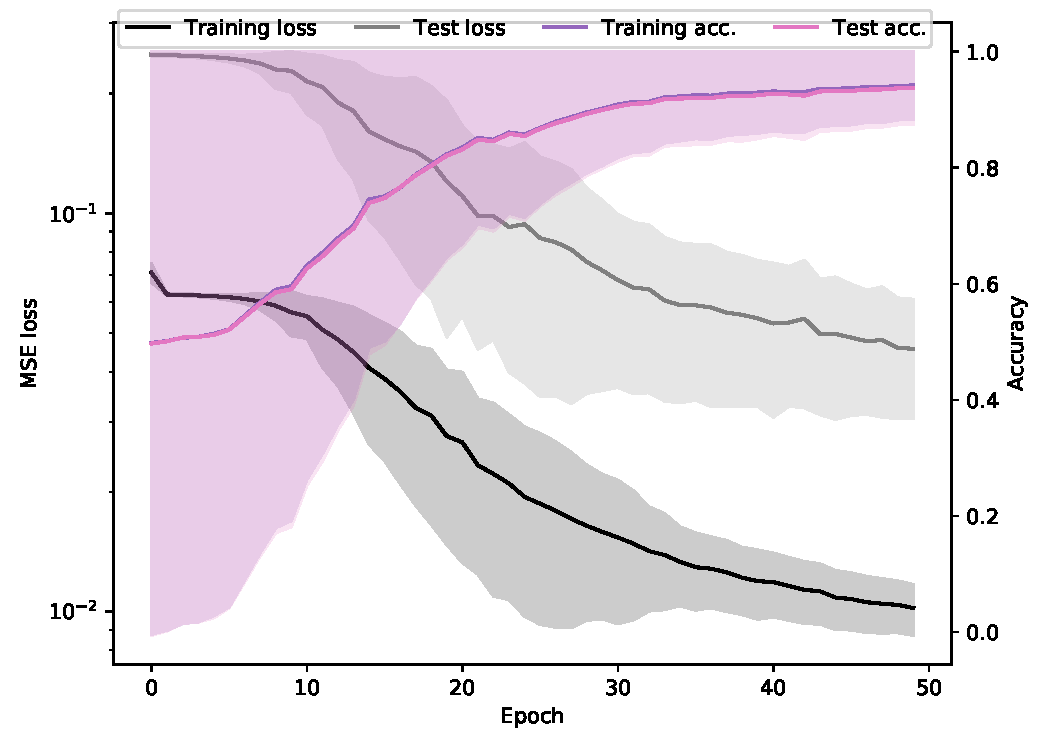
\includegraphics[width=\textwidth]{figures/pytorch/relu_history.pdf}
        \caption{PyTorch ReLU}
    \end{subfigure}
    \begin{subfigure}[]{0.45\linewidth}
        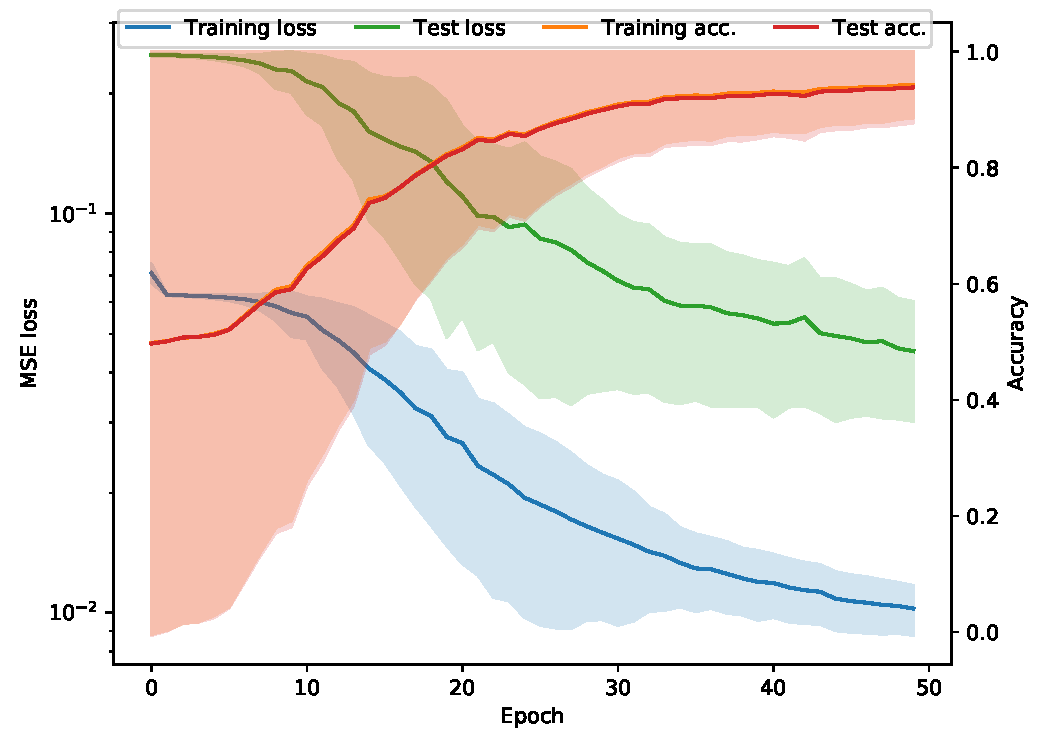
\includegraphics[width=\textwidth]{figures/mini/relu_history.pdf}
        \caption{Mini ReLU}
    \end{subfigure}
    \begin{subfigure}[]{0.45\linewidth}
        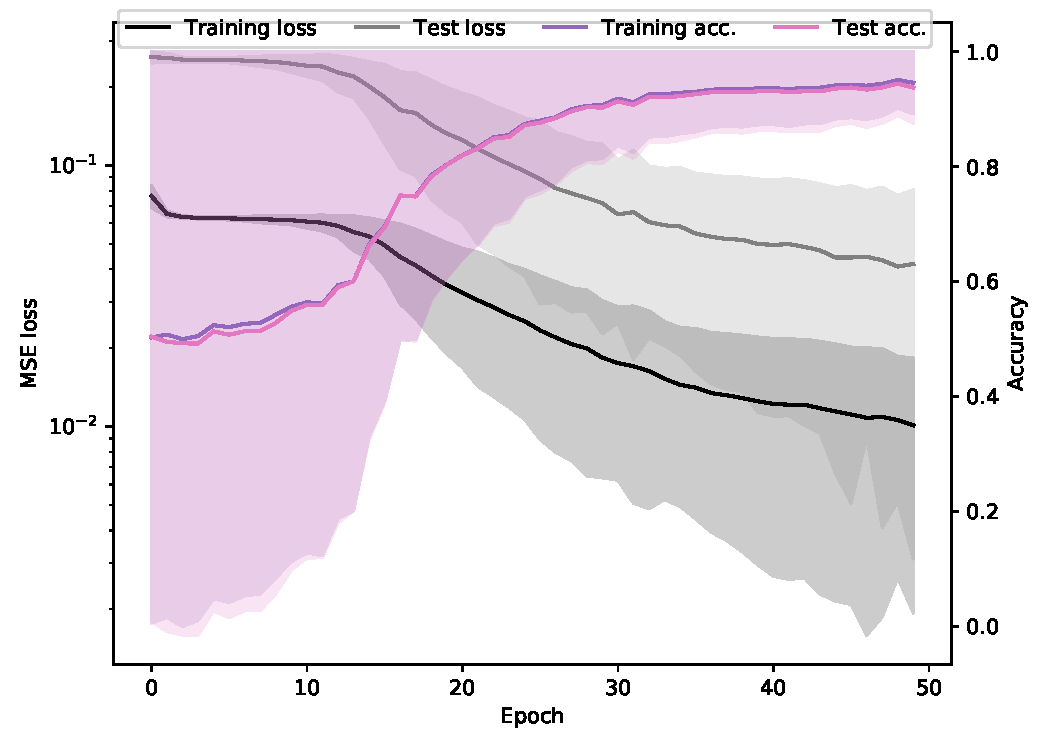
\includegraphics[width=\textwidth]{figures/pytorch/tanh_history.pdf}
        \caption{PyTorch tanh}
    \end{subfigure}
    \begin{subfigure}[]{0.45\linewidth}
        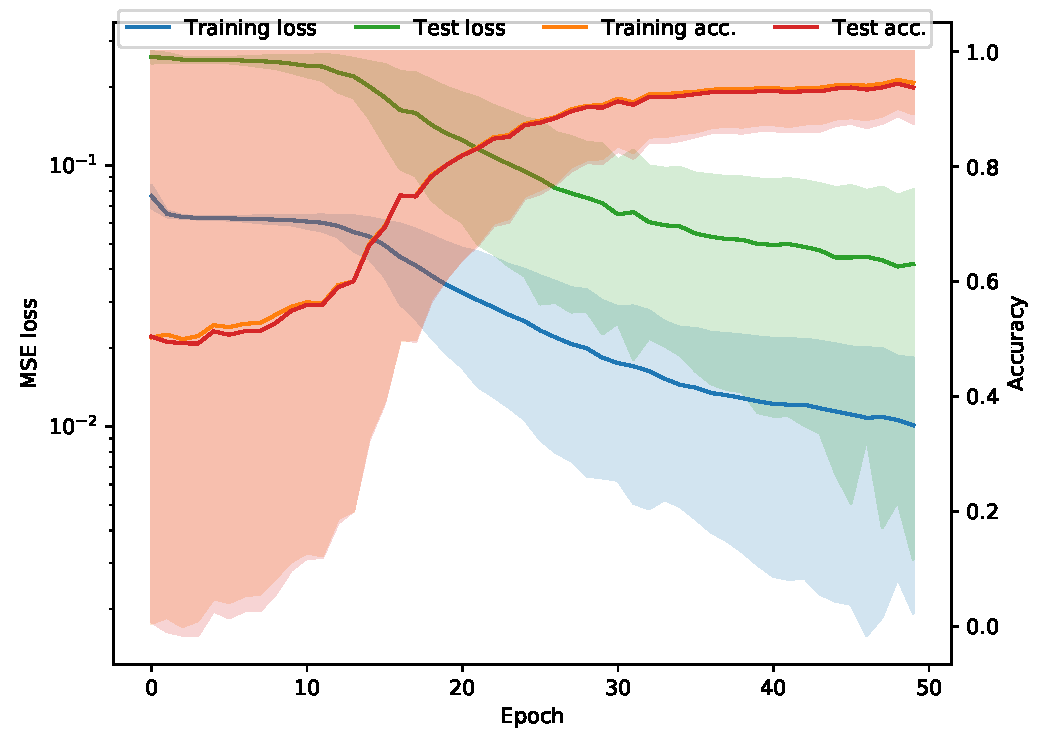
\includegraphics[width=\textwidth]{figures/mini/tanh_history.pdf}
        \caption{Mini tanh}
    \end{subfigure}
    \caption{Average training curves for ReLU and tanh activation using PyTorch and the mini deep-learning framework presented in this report ($N=32$)}
    \label{fig:training}
\end{figure}

\begin{figure}[h!]
    \begin{subfigure}[]{0.45\linewidth}
        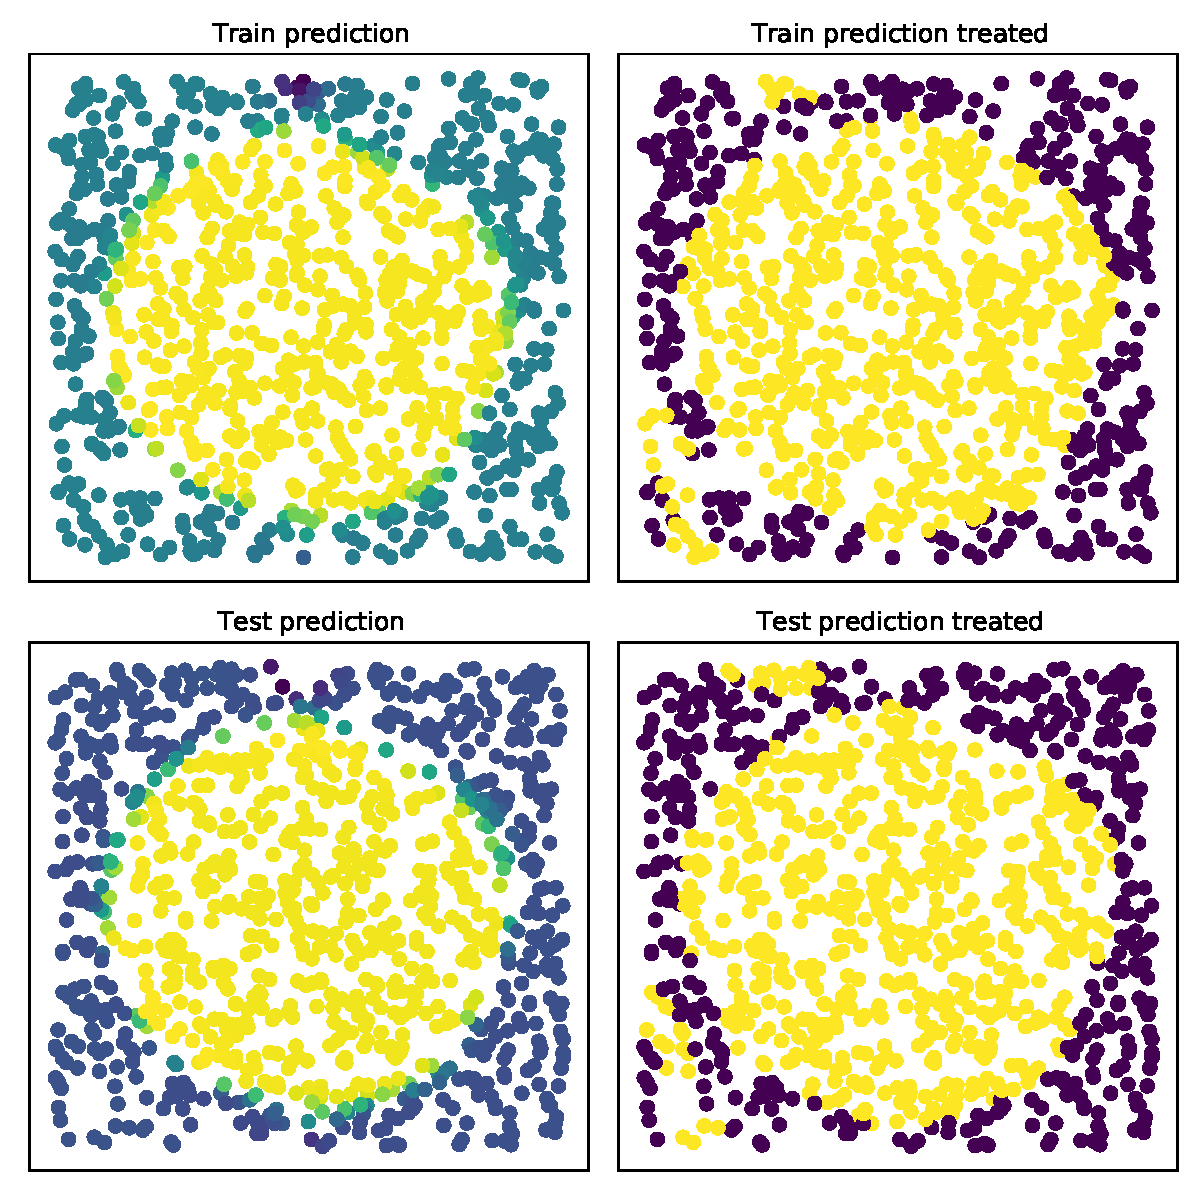
\includegraphics[width=\textwidth]{figures/tanh_points.pdf}
        \caption{tanh}
    \end{subfigure}
    \begin{subfigure}[]{0.45\linewidth}
        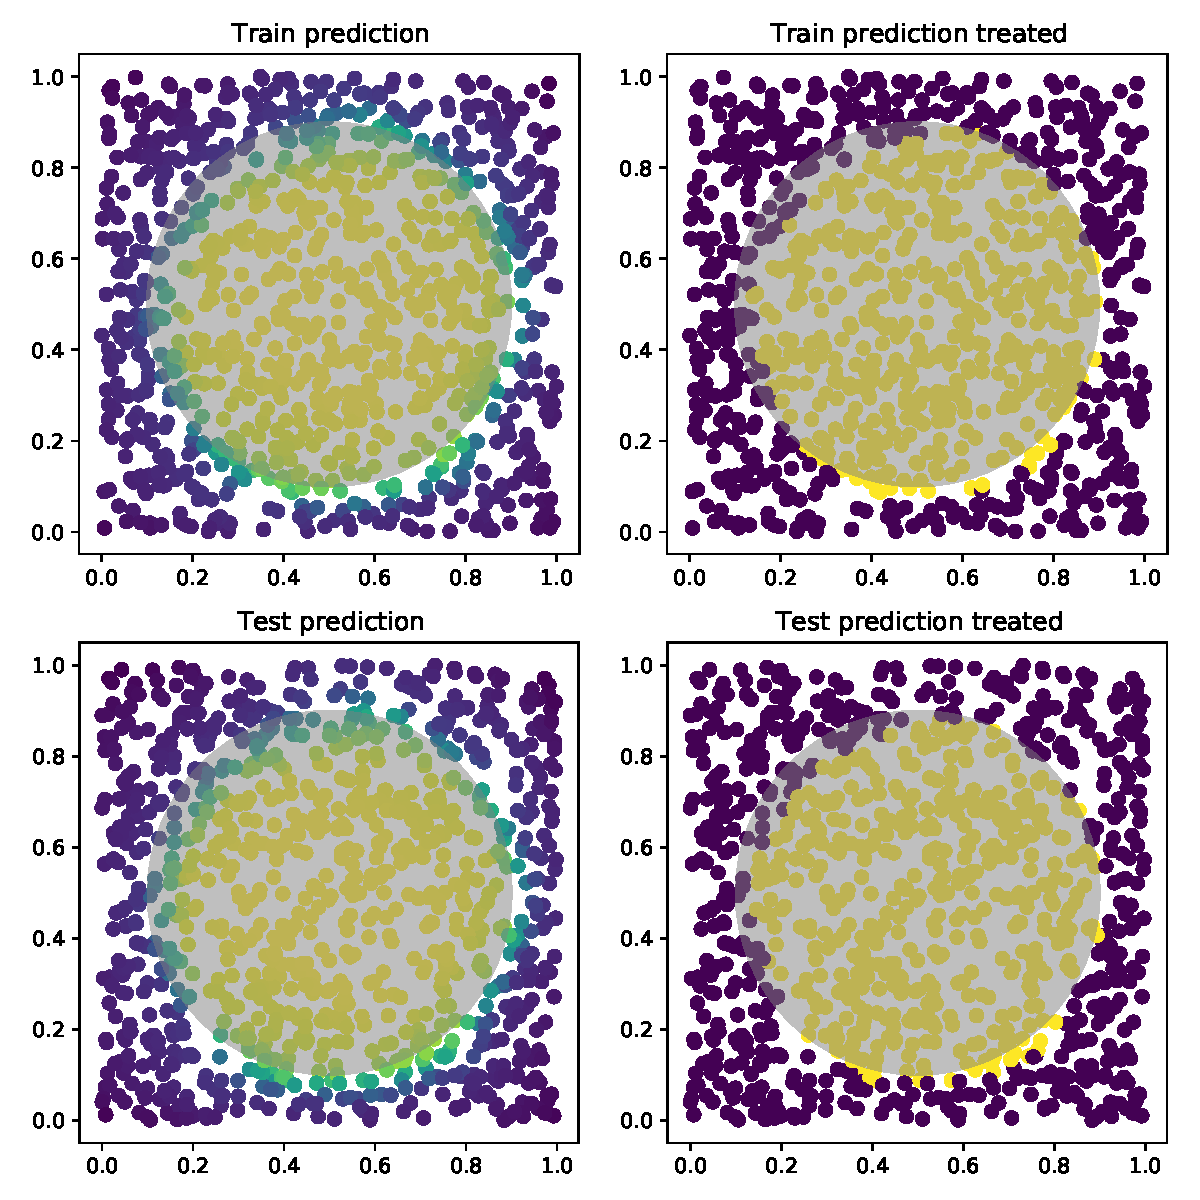
\includegraphics[width=\textwidth]{figures/relu_points.pdf}
        \caption{ReLU}
    \end{subfigure}
    \caption{The left subplots of the subfigures are colored by the direct output of the mini framework model; the right subplots are colored by the rounded tanh of the model outputs. The top subplots of the subfigures are training data; the bottom are test data.}
    \label{fig:points}
\end{figure}

\section{Conclusions}


\end{document}